\documentclass{article}
\usepackage[utf8]{inputenc}
\usepackage{romannum}
\usepackage{amsfonts}
\usepackage{amssymb}
\usepackage{fancyhdr}
\usepackage{graphicx}
\usepackage{t1enc}
\usepackage{pdfpages}
\usepackage[magyar]{babel}
\usepackage[utf8]{inputenc}
\usepackage{amsmath}
\usepackage{mathtools}
\usepackage{pdfpages}
\usepackage{ marvosym } 
\usepackage{wrapfig}
\usepackage{hyperref}
\usepackage{pgfplots}

\pgfplotsset{width=\textwidth,compat=newest}
\hypersetup{
    colorlinks,
    citecolor=black,
    filecolor=black,
    linkcolor=black,
    urlcolor=black
}
\usepackage{romannum}
\usepackage{amsfonts}
\usepackage{amssymb}
\usepackage{fancyhdr}
\usepackage{graphicx}
\usepackage{t1enc}
\usepackage{svg}
\usepackage[magyar]{babel}
\usepackage[left=2cm,right=2cm,top=2cm,bottom=2cm]{geometry}

\title{K+F Projekt dokumentáció}
\author{}
\date{2}
\pagestyle{fancy}
\lhead{K+F Projekt dokumentáció}
\rhead{ACSG Kft.}
\cfoot{\thepage. oldal}

\begin{document}
\pagenumbering{arabic}

\begin{center}
    \hrule
    \vspace{0.5cm}
    \begin{Huge}
    K+F projekt dokumentáció\\
    ACSG Kft.\\
    \end{Huge}
    \vspace{0.5cm}
    \begin{huge}
    Időszak:\\
    \end{huge}
    \begin{Large}
    2023.03.01. - 2023.04.30.\\
    \end{Large} \vspace{10pt}
    \begin{large}
    Készítette: Wenesz Dominik\\
    \end{large}\vspace{0.5cm}
    \hrule
    
  \end{center}
  \begin{figure}[b]
    \centering
    
\includegraphics[]{acsg.png}
\end{figure}
  


\thispagestyle{empty}
\setcounter{page}{0}




\newpage
\tableofcontents
\newpage

\section{Mérföldkövek}
A hagyományos objektumdetektáláson alapuló módszereket elvetettük, mint
opciót a projekt megoldására.\\[3pt]
Sikerült kiválasztani a csatlakozóházakhoz megfelelően univerzális,
kompakt végberendezés típust.\\[3pt]
A Deep learningen alapuló objektumdetektálási módszerekkel sikeresen 
tudunk detektálni több osztályhoz tartozó objektumokat.\\[3pt]
A Deep learning nagy adatigényét kielégítő, ipari környezetbe flexibilisen illeszkedő
adatgeneráló szoftvert sikerült kialakítani (GUI még nem teljes).
\section{Összefoglaló}
A dokumentum által tárgyalt időszakban a deep learning alapú objektumdetektálási és
pozíciómeghatározási rendszer véglegesítése zajlott (zajlik), egyúttal megkezdtük a valós 
környezetben, az edge device-on való teszteléseket is.\\[5pt]
Egyúttal a GUI és az azt kiszolgáló háttérrendszer fejlesztése is megkezdődött, melyben először a tetszőleges 
3D CAD modelből egyszerűen történő tanítóadat generálás, valamint az ezen adatokon 
történő neurális háló tanítása, elátrolása, illetve az edge device-ra történő
hálózaton keresztüli feltöltés valósul meg.\\[5pt]
(...)


\section{Objektum detektáló alrendszer}
\subsection{Rendszer gyártókörnyezetbeli működésének leírása}
Mivel az objektumdetektálás egy kellőképpen működő stádiumban tart, 
ezért célszerű megemlíteni a rendszer tervezett viselkedését, kezelését
röviden.\\[5pt]
\begin{itemize}
  \item A kamerarendszerből kapott jelet a feldolgozóegységen futó 
  szoftver (ami a neurális hálót és a megfelelő algoritmusokat tartalmazza) 
  megállíptja, hogy a munkatér mely koordinátáiban és milye pozícióban helyezkednek 
  el csatlakozóházak, illetve a robot számára melyek a felvehetőek.
  \item A feldolgozóegységből kiadott jel alapján pedig a robot (a 
  robotvezérlőn keresztül) felveszi az objektumot és a kívánt koordinátába és
  orientációba állítja azt. 
  \item A GUI felületen adható meg a kívánt program (csatlakozóház típus, mennyiség stb.),
  illetve ide feltöltve adott CAD file-t megtörténik a tanítóadat generálás
  és az új háló tanítása.
  \item További funkciók részletezése később történik.
\end{itemize}

\subsection{Szöghelyzet meghatározás síkokban}
(...)

\subsection{További fejlesztési irány}
\subsubsection{Adatgenerálás további fejlesztések}
(...)
\subsubsection{Hálóoptimalizálás}
(...)
\subsubsection{Szimulációs implementáció}
(...)
\subsubsection{Orientáció detektálás további vizsgálata, tesztelése}
(...)
\section{Robot manipulátor}
\subsection{Precíziós tesztek}
Tekintve, hogy az objektum detektálás területén a manipulátor számára
felvehetőséget, illetőleg a csatlakozó típusát is megfelelő biztonsággal
meg tudjuk állapítani, így a valóságban való tesztelés is kezdetét veszi 
a következő időszakokban a SCARA robottal. Azonban hiába működik megfelelően
a detektáló rendszerünk, ha a megállapított koordináta és pozíció a 
digitális feldolgozórendszeren (robotvezérlő) az aktuátorokkal nem képes
megfelelő hibahatáron belül pozícionálni a manipulátoron található végberendezést.
Ezen problémaforrás kiküszöbölésére a rendszertesztek előtt szükséges 
önmagában a robotvezérlő és a manipulátor együttes pontosságát mérésekkel
megállapítanunk, jóságát validálnunk.\\[5pt]
Megjegyzendő, hogy a munkaterület eltérő pontjaiban ez igen különböző is
lehet, jellemzően a szingularitási pont(ok), illetve a szélső helyzetekben
és azok környezetében nagyobb pozíciós hibát vét a robot.\\[5pt]
Az ilyen jellegű tesztek szükségességét egyben az is indokolja, hogy
a modellezésből adódó esetleges halmozódó hibát kivédhessük, továbbá 
a rendszerről (gyártócella) készülő digitális iker kellően közelítse
a valóságot.\\[5pt]
Azonban egy-egy ilyen tesztelési folyamat kidolgozása nem egyszerű 
feladat, hiszen mindenképp objektív, meghízható mérésekre van szükségünk.
Továbbá fontos szempont, hogy a mérések lehetséges részeit automatizáljuk,
mivel egy manipulátor teljes munkaterületének többszöri pontossági
feltérképezése rengeteg humán erőforrást igényel.\\[5pt]
Először a megfelelő mérési mód megtalálása, annak validálása, majd 
automatizálásának lehetőségeinek vizsgálata a kitűzött célunk.\\
(...)

\subsection{ROS környezetbeli implementáció}
A ROS (Robot operation system) egy nyílt forráskódú middleware, mellyel
bármilyen robot szimulálható és egyben irányítható is. Előnyei közé 
tartozik, hogy több programozási nyelven (pl.: Python, C++) is programozható,
minden könyvtár implementálva van mindegyik támogatott nyelvi csomagra. 
A magasszintű irányítástól egészen a bitszintű kezelésig megvalósíthatók
benne a műveletek. A nemrégiben újradolgozott API (ROS 2.x) pedig lehetővé teszi 
a valós idejű robotvezérlést.\\[5pt]
A projekt szempontjából két okból releváns számunka ez a szoftver:
\begin{itemize}
  \item A rendszerről készülő digitális iker egy részét (közvetlen a 
  robotmanipulátor digitális ikrét) el tudjuk benne készíteni, mely 
  valós/majdnem valós időben képes irányítani, optimalizálni a manipulátor
  mozgatását. A kamerarendszerrel és további szenzorokkal kombinálva pedig 
  olyan funkciók ellátására is alkalmas, mint például az ütközés elkerülés.
  \item Másfelől szimulációk futtatására alkalmas környezet biztosít számunkra,
        melyben a robotvezérlésre szolgáló algoritmusokat, szoftverrészeket
        a fizikai robot bevonása nélkül tudjuk tesztelni. Az ilyen valós
        rendszerbeli implementáció előtti virtuális futtatások kiemelkedően fontosak,
        hiszen egyrészt védjük vele az emberi és tárgyi épséget, továbbá 
        a valós időnél gyorsabban, párhuzamosan, valóságban ritkán előforduló,
        nehezen reprodukálható eseteket is meg tudjuk így vizsgálni. Példaképp
        ha valamilyen anomália miatt a programunk hosszú idő után, vagy specifikus
        input kombinációra nem elvárt működést produkál, akkor a valós tezst előtt
        tudjuk észlelni és javítani a problémát.
\end{itemize}
A projekt jelenlegi szakaszában elkezdtük a ROS megismerését, elsajátítását,
illetve ezzel párhuzamosan a használt SCARA robot implementációját is elkezdtük.\\[5pt]
A precíziós tesztek természetesen a ROS renszerben elkészülő modellre 
is vonatkoznak majd.
\begin{figure}[h]
  \centering
  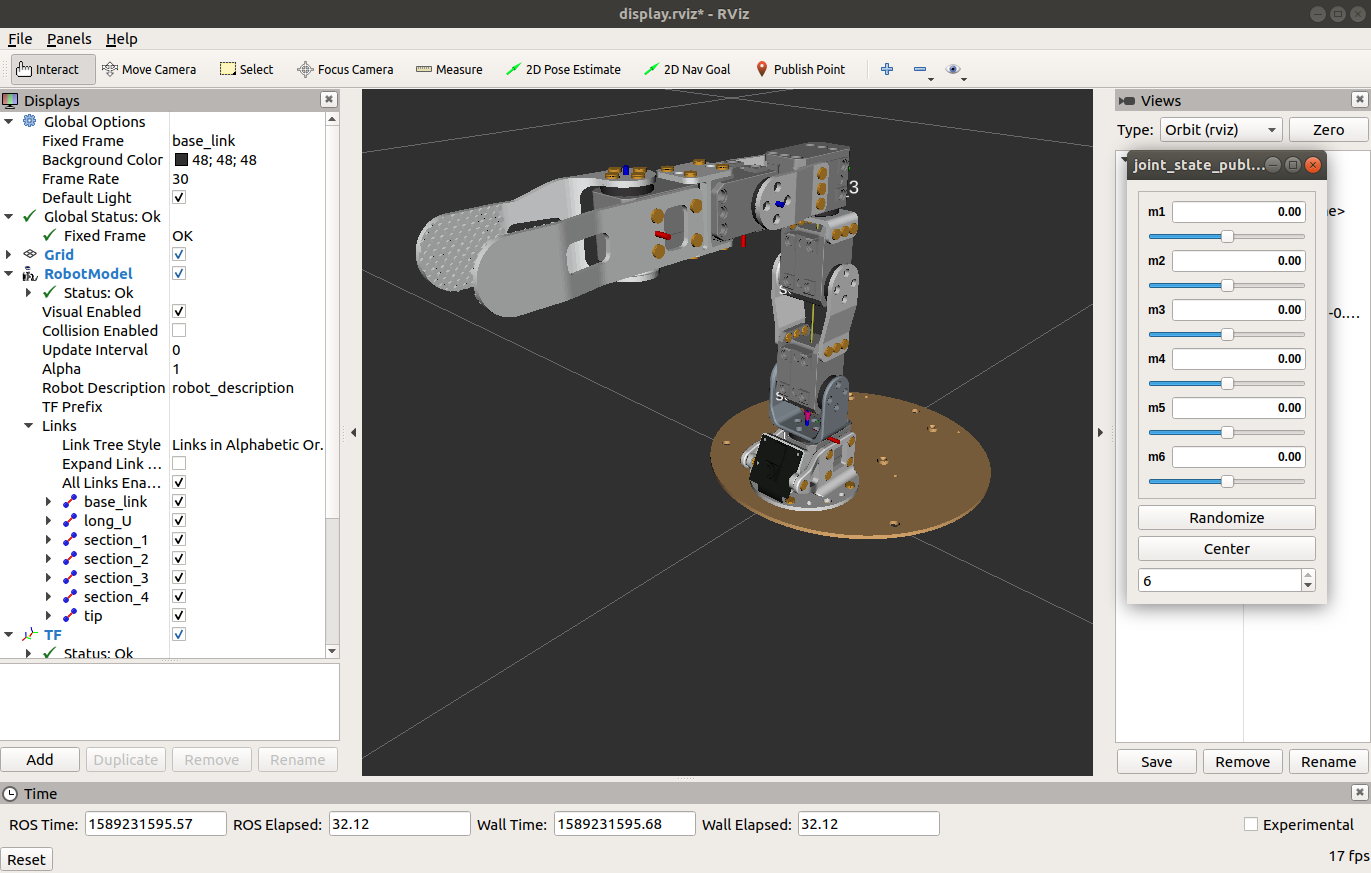
\includegraphics[scale=0.5]{ros_template.png}
  \caption{ROS rendszer mintakép}
\end{figure}\\
(...)
\section{Irodalomjegyzék}







\end{document}